%!TEX root=../documentation-bachlorthesis-speicherarchitektur-lstucker.tex
\cleardoublepage
\chapter{Marktübersicht}

Dieser Abschnitt behandelt den Speichermarkt für primäre Speicher. Mit der Marktübersicht wird einen Überblick verschaffen, welche Speicherlösung Kategorien, Marktsegmente existieren und Hersteller sich im Markt behauptet haben. Zudem wird einen kurzen überblick gegeben, welche Trends im Speichermarkt aktuell sind.

\section{Speicherlösungen}
Die erhältlichen Speicherlösungen lassen sich in die folgenden Kategorien aufteilen: 
\begin{itemize}
\item Konsumer Speicher
\item NAS Speicher
\item Modulare Disk Array Speicher
\item Verteilte Dateisystem Cluster Speicher 
\item Online Speicher auch Cloud Storage genannt.
\end{itemize}

\paragraph*{Konsumer Speicher}
Unter Konsumer Speicher, werden die Speicher für Konsumer Elektronik, wie Notebook, PC, Smartphones, Mulitmedia Center, Audio Player, Camcorder usw. verstanden. Der Speicher basiert vorwiegend auf Blockgeräten wie Festplatten, Flash Disks, Solid State Disk etc.

\paragraph*{NAS Speicher}
NAS Produkte sind gemäss Gartner Speichersysteme, welche mit optimierten Dateisystemen gemeinsamen Dateizugriff für die im LAN angeschlossenen heterogenen Computer Systeme ermöglichen. Die NAS Produkte können ihren Speicher von internen Disks oder Direct-Attached Storage sowie von SAN Array Speicher zur Verfügung stellen. Die NAS Produkte verwenden für den gemeinsamen Dateizugriff Industrie Standardprotokolle, wie zB. Network File System (NFS) in Unix Umgebungen, oder Common Internet File System (CIFS) für Windows-Umgebungen. 
Viele NAS Produkte unterstützen heute natives ISCSI und in einigen Fällen Fibre Channel, um den Speicher auch über Logical Units zur Verfügung zu stellen. Die NAS Produkte werden mit einem für ihre Aufgaben optimierten Betriebsystem betrieben. \cite{RogerW.CoxPushanRinnenStanleyZaffos2011}

\paragraph*{Modulare Disk Array Speicher}
Modulare Disk Array Speicher sind Speichersysteme mit doppelten Controllern oder Node Cluster Architektur, welche den Speicher über Block Zugriffsprotokolle wie Fibre Channel oder ISCSI zur Verfügung stellen. Sie werden mit vom Hersteller vorkonfigurierten Festplatten ausgeliefert. Die Festplatten werden mit eigener Konfiguration oder mittels Konfiguration des Herstellers für die gewünschte Redundanz im Speichersystem in RAID-Einheiten zusammengefasst. Die Modularen Disk Arrays werden vorwiegend im SAN, manchmal auch im DAS Bereich eingesetzt.

\paragraph*{Verteilte Dateisystem Cluster Speicher}
Verteilte Dateisystemspeicher sind Speicher Cluster, welche den Speicher verteilt über mehrere handelsübliche Computerhardware zu einem grossen Speicher zusammenfassen und diese über eine API Anwendung zur Verfügung stellen. Die gespeicherten Daten werden meist in mehrfacher Redundanz über mehre Cluster Nodes im Speicher Cluster verteilt. Neben wenigen spezialisierten Anbieter werden die meisten verteilten Dateisystem Cluster-Speicher als individuelle Lösungen auf eigener Computer-Hardware betrieben.

\paragraph*{Online Speicher (Cloud Storage)}
Online Speicher, oder Cloud Storage genannt, wird von Gartner als Speichersystem, welches seine verfügbare Kapazität über eine Wide-Area-Network inklusive dem Internet als Dienstleistung zur Verfügung stellt. Als Dienst ist die Speicherkapazität nach oben und nach unten skalierbar und wird nach dem jeweiligen Bedarf des Benutzers verrechnet. Dies ist mit der Versorgung von Strom durch einen Elektrizitätsversorger vergleichbar. \cite{AdamW.Couture2010}

\section{Marktsegment}
Der Speichermarkt kann in die Marktsegmente Heimanwender, Kommerz und Grossdatenanbieter unterteilt werden.

\paragraph*{Heimanwender/ Homeoffice} 
Der Heimanwender hat im Vergleich zu den anderen Marktsegmenten einen geringen Speicherbedarf. Seine Speicherlösungen beschränken sich in der Regel auf den internen Speicher seines Computersystems und seiner Elektronikgeräten. Für Heimanwender, welche einen etwas grösseren Speicherbedarf benötigen, (zum Beispiel Multimedia Inhalte oder Home Office) hat sich ein Markt für einfache NAS Systeme etabliert, welche in der Regel Speicherplatzgrössen bis zu 9 Tebibyte erlauben.


\paragraph*{Kommerz}
Zum Marktsegment 'Kommerz' gehören KMUs und Grossunternehmen in der Sparte Handel, Industrie und Dienstleitung. Diese Anbieter haben einen mittleren bis hohen Bedarf an Speicherkapazität, im Tebibyte Bereich. 

Unternehmen, welche tiefe Anforderungen an die eigene IT-Infrastruktur haben, verwenden ihre Speicherlösungen primär für den gemeinsamen Datenzugriff. 

%Dazu kommen oft NAS Speicherlösungen oder im Server integrierte Speicher zum Einsatz.

Unternehmen mit hohen Anforderungen an die eigene IT-Infrastruktur (zB. Finanzdienstleister), verwenden ihre Speicherlösung für den gemeinsamen Datenzugriff auf Datenbanken und unstrukturierte Daten als hochverfügbare Systemumgebung.

%Die hochverfügbaren Systeme für den Betrieb von grossen relationalen Datenbanken, verwenden Modulare Disk Array Speicher, welche mittels Storage Area Network (kurz SAN) ihren Computersystemen redundant gesicherten Datenspeicher zur Verfügung stellt. Für den gemeinsamen Datenzugriff setzen diese Unternehmen ebenfalls auf NAS Speicherlösungen.

\paragraph*{Grosse Datenanbieter}
Zu den grossen Datenanbieter zählen Webdienstleister wie Google, Facebook, Yahoo, Amazone und Unternehmen aus der Multimedia Industrie wie Pixar Studios, RedBull, aber auch Forschungseinrichtungen wie Cern oder Bibliotheken wie die Amerikanische Library of Congress.
Diese verwalten in ihren Speichern grosse Datenvolumen im Bereich von mehreren hundert Tebibyte bis Exbibyte. 

Für die Speicherung solcher Datenmengen stützen sie sich auf verteilte Dateisystem Cluster Speicher oder hochleistungs NAS Speicherlösungen. 

\section{Gross Datenanbieter}
Gemäss den Anforderungen des Auftraggebers und den beshriebenen Szenarien zählt das zu evaluierende Speichersystem zum Marktsegment der Grossen Datenanbieter. Diese Arbeit und Marktanalyse beschränkt sich deshalb auf dieses Marktsegment.

Demzufolge beschäftigen wir uns mit Speicherlösungen in der Kategorie NAS Speicher, Modulare Disk Array Speicher, Verteilte Dateisystem Cluster Speicher und Online Speicher (Cloud Storage).

\section{Welche Speicherlösungen haben sich im heutigen Markt etabliert, }\label{MarktEtabliert}
%welche Systeme habe sich in jüngster Vergangenheit durchgesetzt und welcher Trend ist zu erwarten?

\paragraph*{NAS Speicherlösungen}
Gartner hat die Anbieter von NAS im mittleren und oberen Marktsegment auf Ihre Marktchancen hin untersucht. Gartner hat diese in Marktführer, Herausforderer, Visionäre und Nichen-Anbieter gegliedert. Es wurden nur Anbieter berücksichtigt, die NAS Lösungen ab einem Preis von 25'000\$ anbieten, die mindestens eines der Protokolle NFS oder CIFS unterstützen und ein Betriebseinkommen von mindestens 5 Millionen Doller ausweisen. 

Als Marktführer wurden Anbieter, welche einen bedeutenden Marktanteil haben, ausreichend Marketing- und Verkaufs-Kapazitäten haben und technologisch führend und innovativ sind.

Als Herausforderer gelten Anbieter mit einem starken Produkt, welche einen namhaften Marktanteil besitzen und über Ressourcen verfügen, diesen ausbauen zu können. Die Anbieter sind jedoch zu wenig Visionär, um sich als Marktführer zu qualifizieren.

Als Visionäre gelten Anbieter, die ein einzigartiges, innovatives Produkte anbieten, welches operationale oder finanziell wichtige End-Benuzter Probleme anspricht, jedoch noch nicht bewiesen haben, einen substantiellen Marktanteil gewinnen zu können.

Als Nischen-Anbieter gelten Hersteller, welche clevere Produkte vermarkten, die auf kundenspezifische Bedürfnisse oder Marktsegmente ausgerichtet sind.

Wie aus der \refabb{abb:MagicQuaderNAS} zu entnehmen ist, stuft Gartner die NetApp dicht gefolgt von EMC als Marktleader ein. Als Herausforderer gilt Oracle und als Visionär gilt BlueArc.

Gartner sieht die Stärken von NetApp darin, dass dieser als einer der wenigen wirklichen Storage Anbieter alle Marktstufen abdeckt und mit Software-Features weiterhin die Messlatte der Industrie vorgibt. NetApp hat seinen Unternehmensgewinn in 2010 stark gesteigert. Zu deren Schwächen gehören, dass in der neuen Version ihrer Betriebsystem-Software noch nicht alle Funktionen von der alten Version integriert werden konnten, welche aber weitgehend zu den allgemein geforderten Features zählen.

Zu den Stärken von EMC zählt Gartner die Übernahme von Isilon's, einem visionären Anbieter, welcher starke Wachstumschancen im traditionellen Datencenter und im Cloud Service Markt hat. Gleichzeitig schwächt die Übernahme von Isilon den Hersteller, weil sich die Produkte nun den Funktionen und Einsatzgebieten überlappen und sich die Kunden fragen, wie der Fahrplan der künftigen Entwicklung aussieht, bevor der Kunde neue Investitionen tätigt.

Zu den Stärken von BlueArc zählt Gartner, dass BlueArc mit Titan und Mercury ein NAS System anbietet, welches hoch-performant und Modular ausbaubar ist. Zu den wichtigsten benötigten Verbesserungen gehören die ultraschnelle objektbasierte Replikation im Katastrophenfall. Als weitere Schwachstelle sieht Gartner zudem den kleinen Marktanteil.

\begin{center}
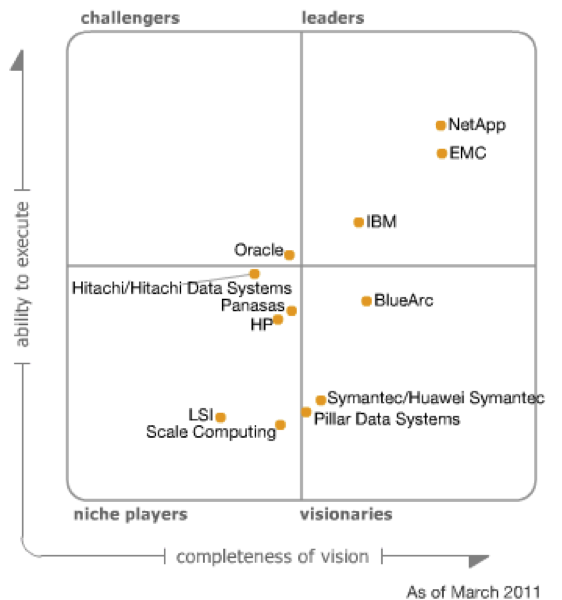
\includegraphics[, keepaspectratio = true]{media/magicquader_nas.png}
\mycaption{figure}{\label{abb:MagicQuaderNAS} Gartner Magic Quader März 2011}
\end{center}

\paragraph*{Modulare Disk Array Speicher}
Gartner hat die Anbieter von Modularen Disk Array im mittleren und oberen Bereich auf deren Marktchancen hin untersucht und hat diese in Marktführer, Herausforderer, Visionäre und Nichen-Anbieter unterteilt. Es wurden nur Anbieter berücksichtig die Modularen Disk Array Lösungen ab einem Preis von 25'000\$ anbieten und in den Märkten Nord Amerika, EMEA oder Japan und Asien Pazifik vertreten sind.

Als Marktführer wurden Anbieter, welche einen bedeutenden Marktanteil haben, ausreichend Marketing- und Verkaufs-Kapazitäten haben und technologisch führend und innovativ sind.

Als Herausforderer gelten Anbieter mit einem starken Produkt, welche einen namhaften Marktanteil besitzen und über Ressourcen verfügen, diesen ausbauen zu können. Die Anbieter sind jedoch zu wenig Visionär, um sich als Marktführer zu qualifizieren.

Als Visionäre gelten Anbieter, die ein einzigartiges, innovatives Produkte anbieten, welches operationale oder finanziell wichtige End-Benuzter Probleme anspricht, jedoch noch nicht bewiesen haben, einen substantiellen Marktanteil gewinnen zu können.

Als Nischen-Anbieter gelten Hersteller, welche clevere Produkte vermarkten, die auf kundenspezifische Bedürfnisse oder Marktsegmente ausgerichtet sind.

Wie aus der \refabb{abb:MagicQuaderModularDiskarrays} zu entnehmen ist, stuft Gartner EMC, NetApp, HP, Dell und Hitachi Data System zu den Marktführern ein. Oracle und Fujitsu sieht Gartner als Herausforderer und XIO wird als visionär bezeichnet.
 
\begin{center}
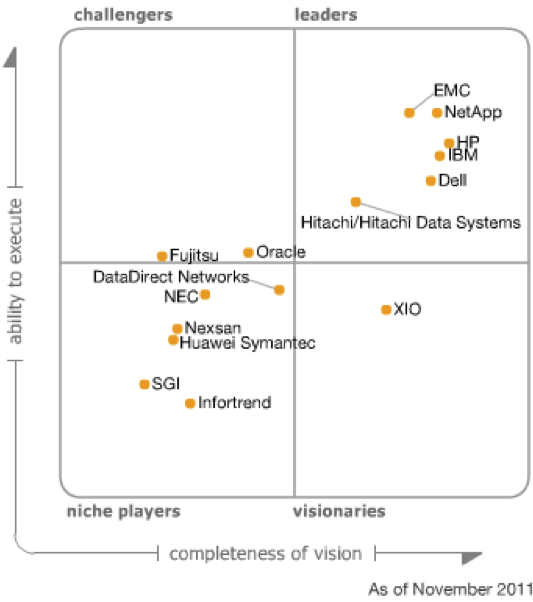
\includegraphics[, keepaspectratio = true]{media/magicquader_modulardiskarrays.png}
\mycaption{figure}{\label{abb:MagicQuaderModularDiskarrays} Gartner Magic Quader Modular Disk ArrayMärz 2011}
\end{center}


\paragraph*{Distributed Filesystem Cluster Speicherlösungen}
Zu den bekannten Vertreter der Distributed Filesystems gehören Hadoop HDFS, Gluster, Lustre. Alle drei haben gemeinsam, dass es sich bei den Lösungen um Open-Source Software handelt.

Hadoop basiert auf dem Design-Konzept von Google Filesystem und Google Mapreduce. The Guardian hat Apache Hadoop 2011 als Erfinder des Jahres ausgezeichnet. InfoWorld hat Hadoop für den InfoWorld 2012 Technology Award gewählt und für Gartner zählt Hadoop zu den top 10 Technologie-Trends, welche Einfluss auf die Informatik Infrastruktur nehmen. 
Zu dem prominentesten Unternehmen die Hadoop einsetzen und mitentwickeln zählen Yahoo und Facebook. Neben den beiden genannten gibt es mtllerweile viele weitere namhafte Unternehmen wie IBM, AOL, Twitter die Hadoop einsetzen. \cite{Guardian}\cite{Wayner2012}\cite{Casonato2012}\cite{Hadoop2012}

GlusterFS wurde von der Firma Gluster Inc. als Opensource Projekt entwickelt. Im Jahr 2011 wurde GlusterInc von der Firma Red Hat Inc. übernommen, um Lösungen für den Big Data Bereich anbieten zu können. Red Hat wurde mit der Übernahme von Gluster Inc zum Hauptunterstützer von GlusterFS.

\paragraph*{Online Speicher}
Einer der ersten grossen und wohl der bekannteste Online Speicher Anbieter zählt Amazone mit ihrem S3 Produkt. Amazone veröffentlicht zwar keine Finanzdaten über ihre Cloud Produkte, hingegen veröffentlichte Amazon Daten bezüglich dem Wachstum der Anzahl gespeicherten Objekten. Gemäss eigenen Aussagen speicherte Amazon im Jahr 2006 ca. 2.9 Milliarden Objekte, im Jahr 2010 wahren es bereits 269 Milliarden Objekte. Dieses Ergebnis könnte Amazon im Jahr 2011 mit 762 Milliarden Objekten mehr als verdoppeln. \cite{Barr2012}

\begin{center}
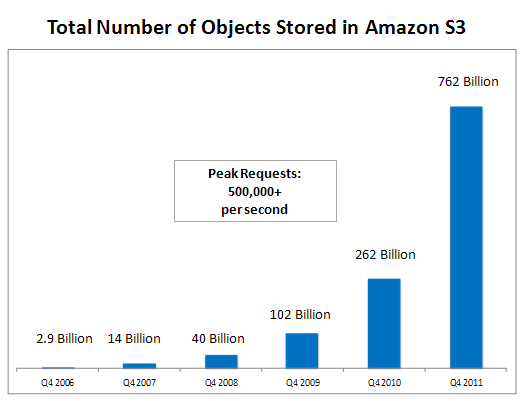
\includegraphics[, keepaspectratio = true]{media/s3_growth_2011_3.png}
\mycaption{figure}{\label{abb:MagicQuaderModularDiskarrays} 
\cite{Barr2012}Anzal gespeicherte Objekte in Amazon S3 \cite{Barr2012}}
\end{center}

Neben Amazon zählt RackSpace zu den führenden Cloud Anbietern. Wie Amazon bietet auch RackSpace den Online Speicher für jedermann an. Ihr Online Speicher wird unter der Produkt Bezeichnung Cloud File vermarktet. Hinter Cloud File steckt ein selbst entwickelter Speicher, OpenStack Object Storage mit Code Name Swift genannt. RackSpace hat an OpenStack Object Storage ein Jahr lang entwickelt und diese wie ihre anderen Cloud Eigenentwicklungen als Quelloffenes Projekt unter OpenStack veröffentlicht. Zu OpenStack tragen neben Rackspace weitere nahmhafte Unternehmen wie \gls{Dell}, \gls{HP}, Citrix, AMD, NetApp, Suse, AT\&T, NASA und andere bei.
RackSpace setzt ferner den selbst entwickelten OpenStack Object Storage als Online Speicher ein. \cite{OpenStack}

In der Schweiz ist die Entwicklung von Cloud Storage noch nicht so weit fortgeschritten wie in Amerika. Zu den wenigen Anbietern gehört unter anderem die Swisscom.


\section{Trend}
Für Gartner zählen Modular Disk Array Speicher und NAS zu den etablierten Speicherlösungen. Online Speicher (Cloud Storage) sieht Gartner eher als Speicherlösungen der Zukunft, welche sie laufend beobachtet und einen festen Platz in ihren Marktanalysen bekommen hat. 


%weshalb wiso warum

% wenig anbieter welche grosse datenanbieter 

% statistic massendaten